\normaltrue \difficilefalse \tdifficilefalse
\correctionfalse
%\UPSTIidClasse{11} % 11 sup, 12 spé
%\newcommand{\UPSTIidClasse}{11}

\exer{Système EPAS $\star$ \label{B2:16:64}}
%% CCP MP 2007
\setcounter{numques}{0}
\UPSTIcompetence[2]{B2-16}
\index{Compétence B2-16}

\index{EPAS}
\index{Hyperstatisme}

\ifcorrection
\else
\textbf{Pas de corrigé pour cet exercice.}
\fi

\ifprof
\else
On s'intéresse à l'échelle pivotante équipant un camion de pompier.


\begin{center}
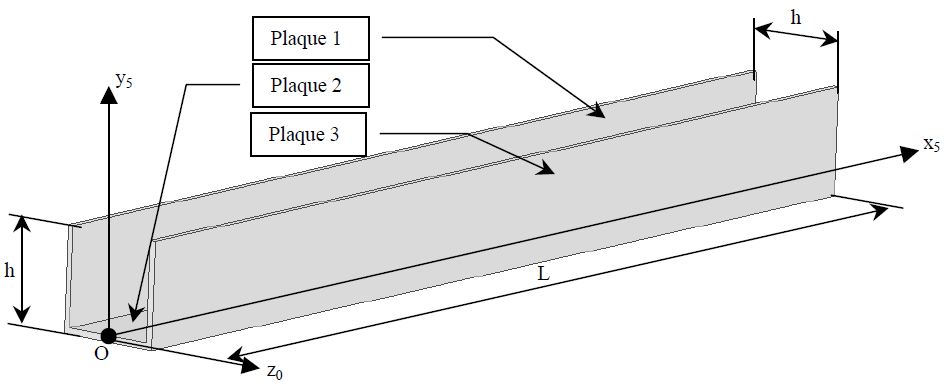
\includegraphics[width=8cm]{64_01}
\end{center}

On donne un schéma cinématique du système de manoeuvre du parc échelle.

\begin{center}
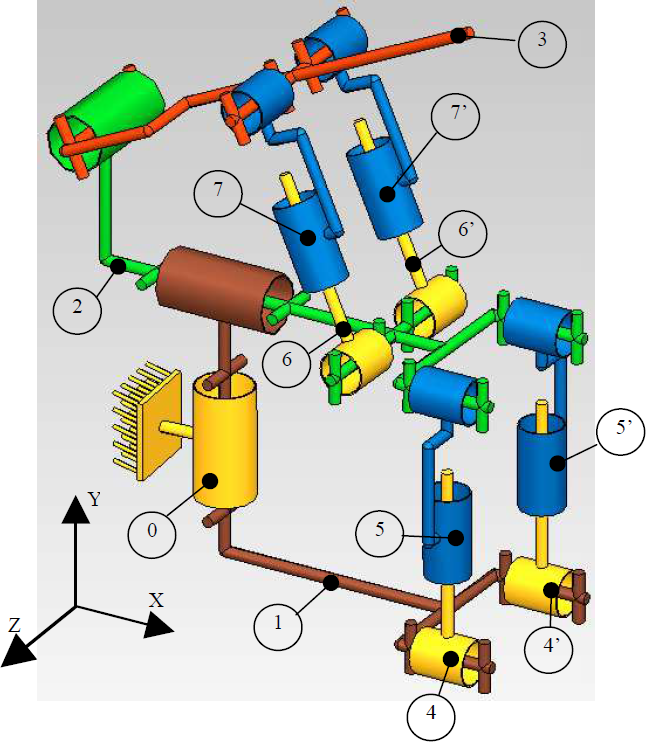
\includegraphics[width=8cm]{64_02}
\end{center}

\fi

\question{Réaliser le graphe des liaisons.}
\ifprof

\begin{center}
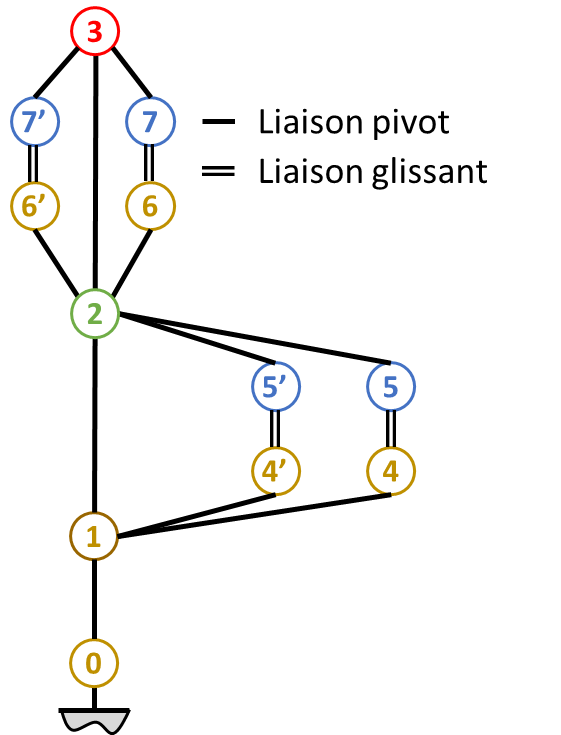
\includegraphics[width=10cm]{64_01_cor}
\end{center}

\else 
\fi

\question{Déterminer le degré d’hyperstatisme de ce mécanisme.}
\ifprof
Détermination des mobilités : 
\begin{itemize}
\item rotation de l'ensemble des pièces en rotation autour de $\vect{y}$ grâce à la pivot entre 0 et 1;
\item rotation de la pivot entre 1 et 2 par mouvements opposés des pivots glissant 4--5 et 4'--5';
\item rotation de la pivot entre 2 et 3 par mouvements simultanés des pivots glissant 6--7 et 6'--7'.
\end{itemize}
On a donc $m=3$. 

\textbf{Méthode cinématique : }
\begin{itemize}
\item nombre de cycles : 15 liaisons et 12 solides, $\gamma = L- S + 1 =4$;
\item nombre d'équations cinématiques: $E_c = 6\times 4 = 24$;
\item nombre d'inconnues cinématiques : $I_c = 4 \times 2+ 11 \times 1 = 19$;
\item hyperstaticité : $h=m-I_c + E_c = 3 -19 + 24 = 8$.
\end{itemize}


\textbf{Méthode statique : }
\begin{itemize}
\item nombre d'équations statiques : $E_s = 6\times 11 = 66$;
\item nombre d'inconnues statiques : $I_s = 4 \times 4+ 11 \times 5 = 71$;
\item hyperstaticité : $h=m-E_s + I_s = 3 -66 + 71 = 8$.
\end{itemize}


\else 
\fi

\question{Proposer des modifications qui permettraient de le rendre isostatique.}
\ifprof
On va chercher à rendre le système isostatique tout en conservant une même architecture pour des branches en parallèles.
%
%Dans le cycle 1--4--5--2--5'--4'--1 pris indépendamment du reste du mécanisme on a :
%\begin{itemize}
%\item $m=2$;
%\item $I_c = 8$;
%\item $E_c =6 \times 1$;
%\item $h = m-I_c +E_c = 2 -8 +6 = 
%\end{itemize}

\else 
\fi
 
 

\ifprof
\else
\ifcolle
\else
\noindent\footnotesize
 \fbox{\parbox{.9\linewidth}{
 Éléments de corrigé : 
 \begin{enumerate}
\item .
\item $h=8$.
\item .
 \end{enumerate}}}
\normalsize
\fi

\begin{flushright}
\footnotesize{Corrigé  voir \ref{B2:16:64}.}
\end{flushright}%
\fi